%%%%%%%%%%%%%%%%%%%%%%%%%%%%%%%%%%%%%%%%%%%%%%%%%%%%%%%%%%%%%%%%%%%%%%
% amspaper.tex --  LaTeX-based template for submissions to American 
% Meteorological Society journals
%
% Template developed by Amy Hendrickson, 2013, TeXnology Inc., 
% amyh@texnology.com, http://www.texnology.com
% following earlier work by Brian Papa, American Meteorological Society
%
% Email questions to latex@ametsoc.org.
%
%%%%%%%%%%%%%%%%%%%%%%%%%%%%%%%%%%%%%%%%%%%%%%%%%%%%%%%%%%%%%%%%%%%%%
% PREAMBLE
%%%%%%%%%%%%%%%%%%%%%%%%%%%%%%%%%%%%%%%%%%%%%%%%%%%%%%%%%%%%%%%%%%%%%

%% Start with one of the following:
% DOUBLE-SPACED VERSION FOR SUBMISSION TO THE AMS
\documentclass{ametsoc}

% TWO-COLUMN JOURNAL PAGE LAYOUT---FOR AUTHOR USE ONLY
% \documentclass[twocol]{ametsoc}

%%%%%%%%%%%%%%%%%%%%%%%%%%%%%%%%
%%% To be entered only if twocol option is used

%\journal{jcli}

\usepackage{color}

%  Please choose a journal abbreviation to use above from the following list:
% 
%   jamc     (Journal of Applied Meteorology and Climatology)
%   jtech     (Journal of Atmospheric and Oceanic Technology)
%   jhm      (Journal of Hydrometeorology)
%   jpo     (Journal of Physical Oceanography)
%   jas      (Journal of Atmospheric Sciences)	
%   jcli      (Journal of Climate)
%   mwr      (Monthly Weather Review)
%   wcas      (Weather, Climate, and Society)
%   waf       (Weather and Forecasting)
%   bams (Bulletin of the American Meteorological Society)
%   ei    (Earth Interactions)

%%%%%%%%%%%%%%%%%%%%%%%%%%%%%%%%
%Citations should be of the form ``author year''  not ``author, year''
\bibpunct{(}{)}{;}{a}{}{,}

%%%%%%%%%%%%%%%%%%%%%%%%%%%%%%%%

%%% To be entered by author:

%% May use \\ to break lines in title:

\title{}

%change the title?

%%% Enter authors' names, as you see in this example:
%%% Use \correspondingauthor{} and \thanks{Current Affiliation:...}
%%% immediately following the appropriate author.
%%%
%%% Note that the \correspondingauthor{} command is NECESSARY.
%%% The \thanks{} commands are OPTIONAL.

  
%%%%%%%%%%%%%%%%%%%%%%%%%%%%%%%%%%%%%%%%%%%%%%%%%%%%%%%%%%%%%%%%%%%%%
% ABSTRACT
%
% Enter your Abstract here

%\abstract{} 

\begin{document}


%% Necessary!
%\maketitle


\section{Preliminary analyses}

Based on the WRF datasets referred by Daniel, I have looked into the relevant changes of precipitation (focused on winter season) from the past (year 1991-2000) to the future (presumably year 2091-2100). Here are some initial investigation (mainly in the qualitative aspect) with supported rough plots attached.\\

1) How well does WRF reproduce the historical mean precipitation compared to observations (here, only show PRISM)?

As shown in the plot (see Figure \ref{fig:Figure 1}), WRF performed quite good compared to PRISM, although there are notable biases over the mountain peaks as the grid resolution increased to 3 km.\\

2) With the intensified thermodynamic forcing, how precipitation is projected to be changed over California? How about the orographic precipitation over the Sierra Nevada (SN)?

Overall, as climate keeps warming prescribed by RCP 8.5, the ensemble mean Pr from the five selected GCMs is projected to increase moderately mainly over the wet area (i.e. the North coast and mountainous area) (please see Figure \ref{fig:Figure 2} and Figure \ref{fig:Figure 3}). Specifically, within the five models, three show increasing trend with diverse magnitude; The other two show either minor changes or opposite trend over SN. The overall changing trends from the dynamically downscaled results of WRF are consistent with five GCMs' output except for model inmcm4 when referred to Figure 2 in Daniel�s paper about the snowpack \citep{walton2016incorporating}.\\


3) How about the changes of different precipitation events (here, simply dividing into the low-rainy, the high-rainy and the extreme)? To what extent, the changes of these different rainy events contribute to the overall changes of Pr?

When looking at Figure \ref{fig:Figure 4}, it can be found that low-rainy events act as a negative factor to the changes of precipitation in the future from the ensemble mean result over eastern area of the Central Valley and windward of Sierra Nevada. Again, there are inconsistent behaviors within the five models, especially when we compare the GFDL model and the MPI model to the other three remaining models. Particularly, in the GFDL model, there are disorganized signals of the changes, which might be related with the downscaling of the regional wind circulation pattern with unresolved processes.

The high-rainy days have increased and contributed mainly to the mean precipitation increase over the coastal area, the Central Valley, southern part and the relatively low-level of the mountainous regions (see Figure \ref{fig:Figure 5}). However, over the high-level mountainous area, the precipitation changes mainly result from extreme events (see Figure \ref{fig:Figure 6}).

Further, the frequency distribution is roughly conveyed in the Figure \ref{fig:Figure 7}, showing the frequency of the low-rainy, the high-rainy and the extreme over the historical period (i.e. year 1991-2000) and their corresponding contributions to the total rainy amount. This further supports that the precipitation over both dry and wet area over California will tend to be more extreme with the distribution shifts with higher upper tail.\\

4) As the temperature increases in the future, whether the specific humidity will enlarge followed by the Clausius-Clapeyron (C-C) relationship? 

The relative changes of the specific humidity and its relationship to the temperature are given in Figure \ref{fig:Figure 8} and \ref{fig:Figure 9}. Overall the intensity of the specific humidity (Q2) changes is higher over the area where the temperature increases more. Specifically, the proportional changes of the Q2 contrast to the increases of T2 are higher than 7$\%$ over most regions reaching higher than 10$\%$ over the area warms most.

5) How the frequency of different rainy events is predicted to be changed?

First, we look at the relative changes of total rainy days averaged during wet season. The result shows a relative minor changes of rainy days except the lee side of Sierra Nevada (see Figure \ref{fig:Figure 10}). This is pattern is even more obvious for low-rainy days as Figure \ref{fig:Figure 11} shown. In Figure \ref{fig:Figure 11}, the outmost domain is displayed with the middle domain to see how the dynamical downscaling works. It seems that the higher resolution at 9km has more local features and tends to have less low-rainy days with finer topography, although the overall changes of low-rainy days are slight.

For the heavy-rain events (see Figure \ref{fig:Figure 12} and Figure \ref{fig:Figure 13}), the frequency has increased notable over both sides of SN, especial over the dry Central Valley and the lee side, but decreased over the mountain peaks.

%%%%%continued%%%%%%%%%%%

6) How the frequency distribution of daily Pr changes over California from past to future?

First, the 95th quantile (P95) of daily Pr at each grid point has been given here (see Figure \ref{fig:Figure 14}) to show a general picture that whether the upper tail of the Pr distribution has shifted and how. Consistent with previous analyses, there are obvious increases of the P95 for three members (CNRM, INMCM, IPSL) and barely changes for the other two models (GFDL, MPI).

To account for the diverse hydro-climate features over different regions of California (CA), the whole CA has been divided into five zones followed by \cite{huang2016evaluation} (see wrf\_domains.pdf in the folder). From the PDF plot (see Figure \ref{fig:Figure 15}), it can be seen that in the end-century, overall, precipitation is projected to be more extreme over all the regions. Again, discrepancy exists within different model members as aforementioned.


7) The role of large-scale water vapor transport in regulating the heavy-rainy events over California

The integrated water vapor transport (IVT) of the maximum one day Pr (averaged over whole CA) is examined for each simulation to see the track of the water vapor influx during the most heaviest rainy day over CA (see Figure \ref{fig:Figure 16}). Along with the IVT, the near-surface wind pattern and resulted Pr are also given in Figure \ref{fig:Figure 17}, correlating the higher Pr for the future simulations with the increased IVT in the form of atmospheric rivers (ARs) with the warming effect.

Statistically, the average IVT when the mean Pr over whole CA exceeds the P95 is given in Figure \ref{fig:Figure 18}. The P95 value is 14.2 mm/day (averaged over CA), and the number of days with Pr being above P95 are 76, 130, 68, 110, 141 and 96 for hist and other five future simulations. This might give us a general idea of both the thermodynamic (in the aspect of IVT) and dynamic (in the aspect of wind circulation) effects for the future changes of heavy-rainy events. 

As above mentioned, the IVT has notable increased with the warming effect, however, the wind pattern shows diverse changes within different models. Specifically, even the heavy-rainy days have increased largely (30$\%$-85$\%$) within the models (INMCM, IPSL and MPI), the changes of wind patterns tend to play a negative effect with weaken westerly wind. The negative dynamic effect for ARs has also been found by \cite{gao2015dynamical} over western U.S. based on CMIP5 output. For the GFDL model, the IVT has largely increased even with strengthen wind pattern, however, the heavy-rainy days surprisingly show a minor decrease (10$\%$). These changes still hold when using P85 to account for more heavy-rainy events. For reference, the P85 value is 6.9 mm/day, and the number of days with Pr being above P85 are 226, 278, 206, 255, 279 and 229 for hist and other five future simulations.

%Checked the near-surface wind pattern for Maximum 1day Pr, and the wind pattern do show notable difference within the ensemble with resulted discrepancy in the Pr. The wind patterns are similar to the historical average in some GCMs.

%IVT when mean Pr exceeding P90 (Pr =  9.5 mm/day) of hist: 151, 214, 132, 195, 217, 165

\section{Discussions and further directions}

a) The possible reasons that affect the contradictory changes of precipitation within different models.

b) sub-daily Pr dataset

c) hybrid dynamical downscaling

d) The relative change of T vertically over the Sierra Nevada, the condensation rate or cloud liquid water

**check the microphysics in WRF, and how the parameters change the orographic precipitation

notes:

i) Alex: The lee side shows such a large percentage increase. This appears to be coming from the low rainy days, but since precipitation is low there even during large events, this effect may actually be associated with heavy precipitation events in California. This effect seems to be consistent with Stiller and Roe. It would be very interesting to see whether in fact it is.

%a) Dynamical downscaling is necessary for getting more realistic changes of precipitation.
%-> the atmospheric river landings with the corresponding changes of precipitation, like the overlay of different events over different region: This is a bit hard to check at this moment, since the domain is limited and the algorithm to define the AR is remained to be checked. Also, the region devisions need to be recreated for the mask file to separate lee side from windward side

%\acknowledgments

 \bibliographystyle{ametsoc2014}
 \bibliography{database2017}

%Figures

%Figure 1
\begin{figure}
\begin{center}
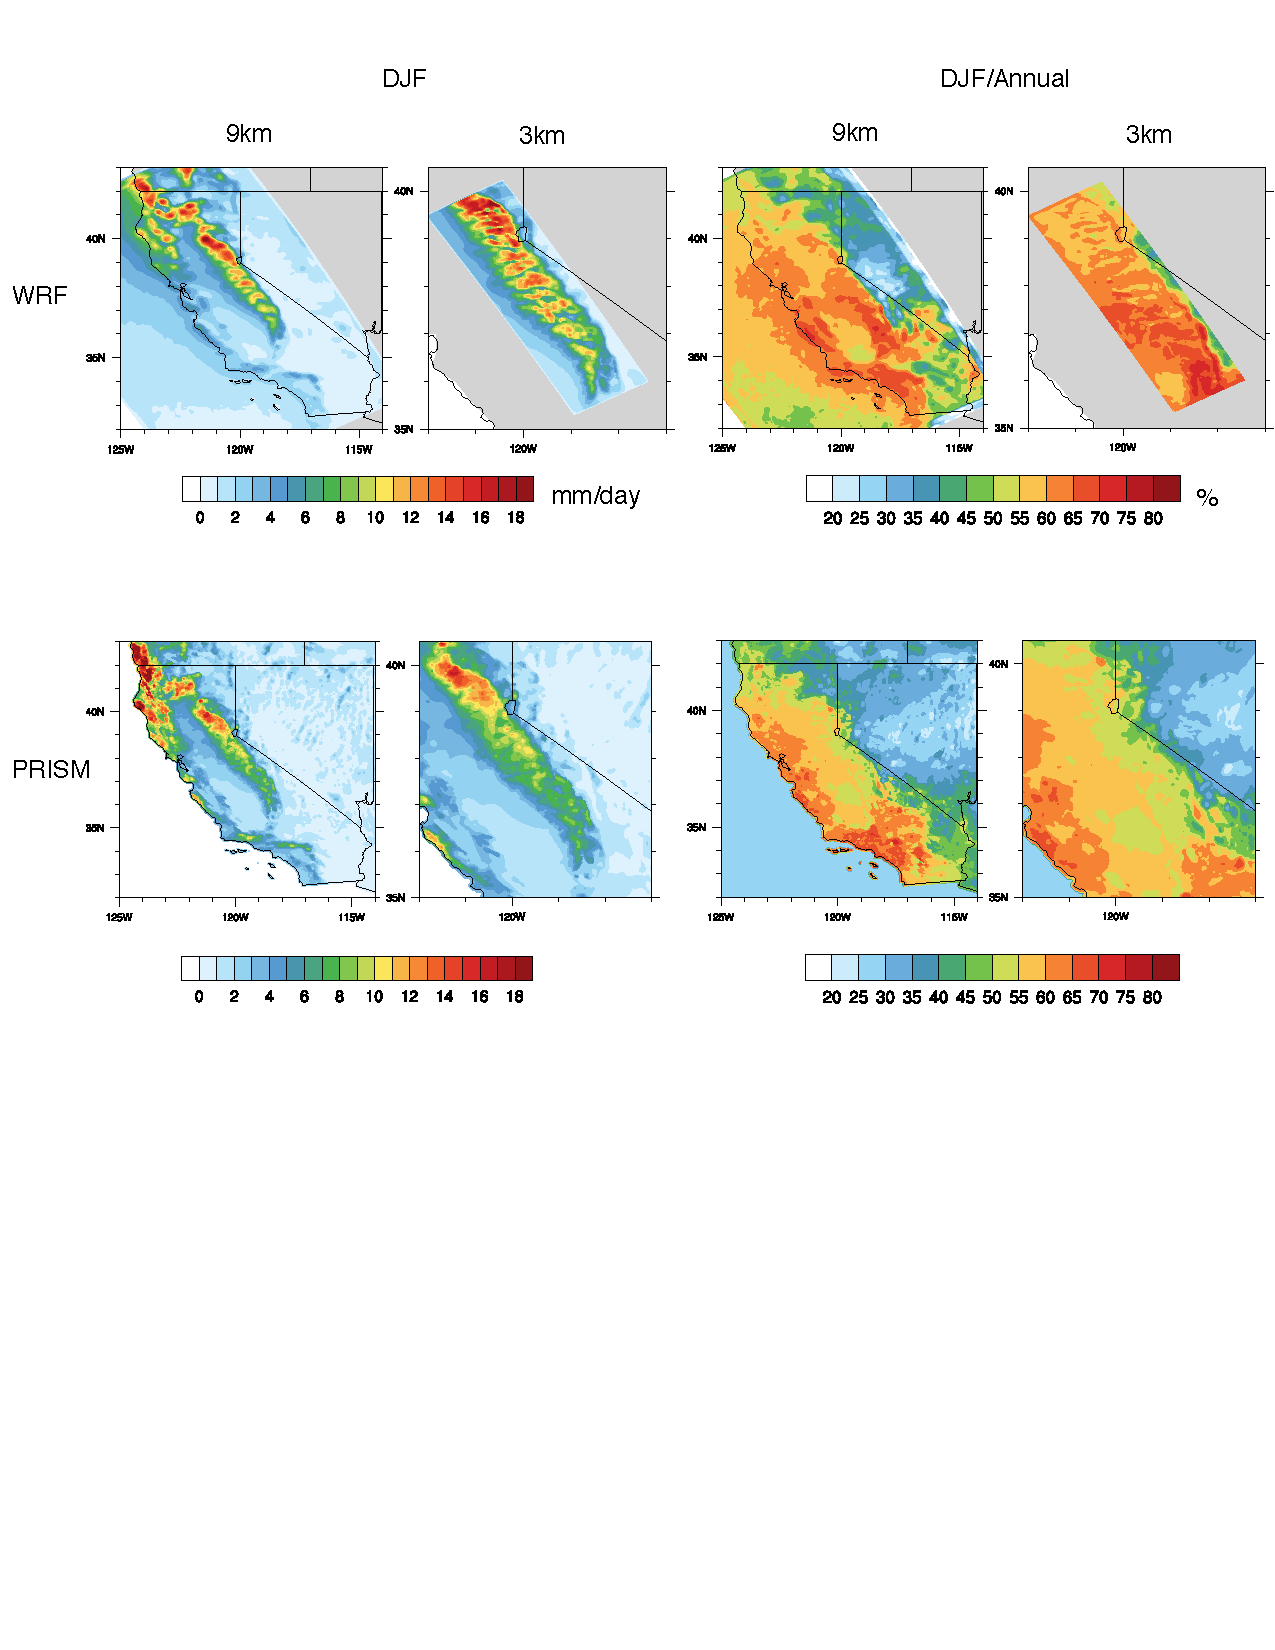
\includegraphics[width=6in]{pr_hist_DJF.pdf}
\caption{The mean DJF precipitation (Pr) and its corresponding contribution to the annual Pr for WRF (9km and 3km) and PRISM, over the historical time period (year 1991-2000).}
\label{fig:Figure 1}
\end{center}
\end{figure}

%Figure 2
\begin{figure}
\begin{center}
\includegraphics[width=6in]{Pr_future-hist_DJF.pdf}
\caption{The changes of mean DJF Pr from the past to future simulated by WRF at 9km and 3km from the five modes and model ensemble mean.}
\label{fig:Figure 2}
\end{center}
\end{figure}

%using NDJFM (i.e. adding november and march) is similar to DJF

%Figure 3
\begin{figure}
\begin{center}
\includegraphics[width=6in]{pr_future_vs_hist_percent_DJF.pdf}
\caption{Similar as Figure 2, but for the relative change in percentage.}
\label{fig:Figure 3}
\end{center}
\end{figure}

%using NDJFM (i.e. adding november and march) is similar to DJF

%Figure 4
\begin{figure}
\begin{center}
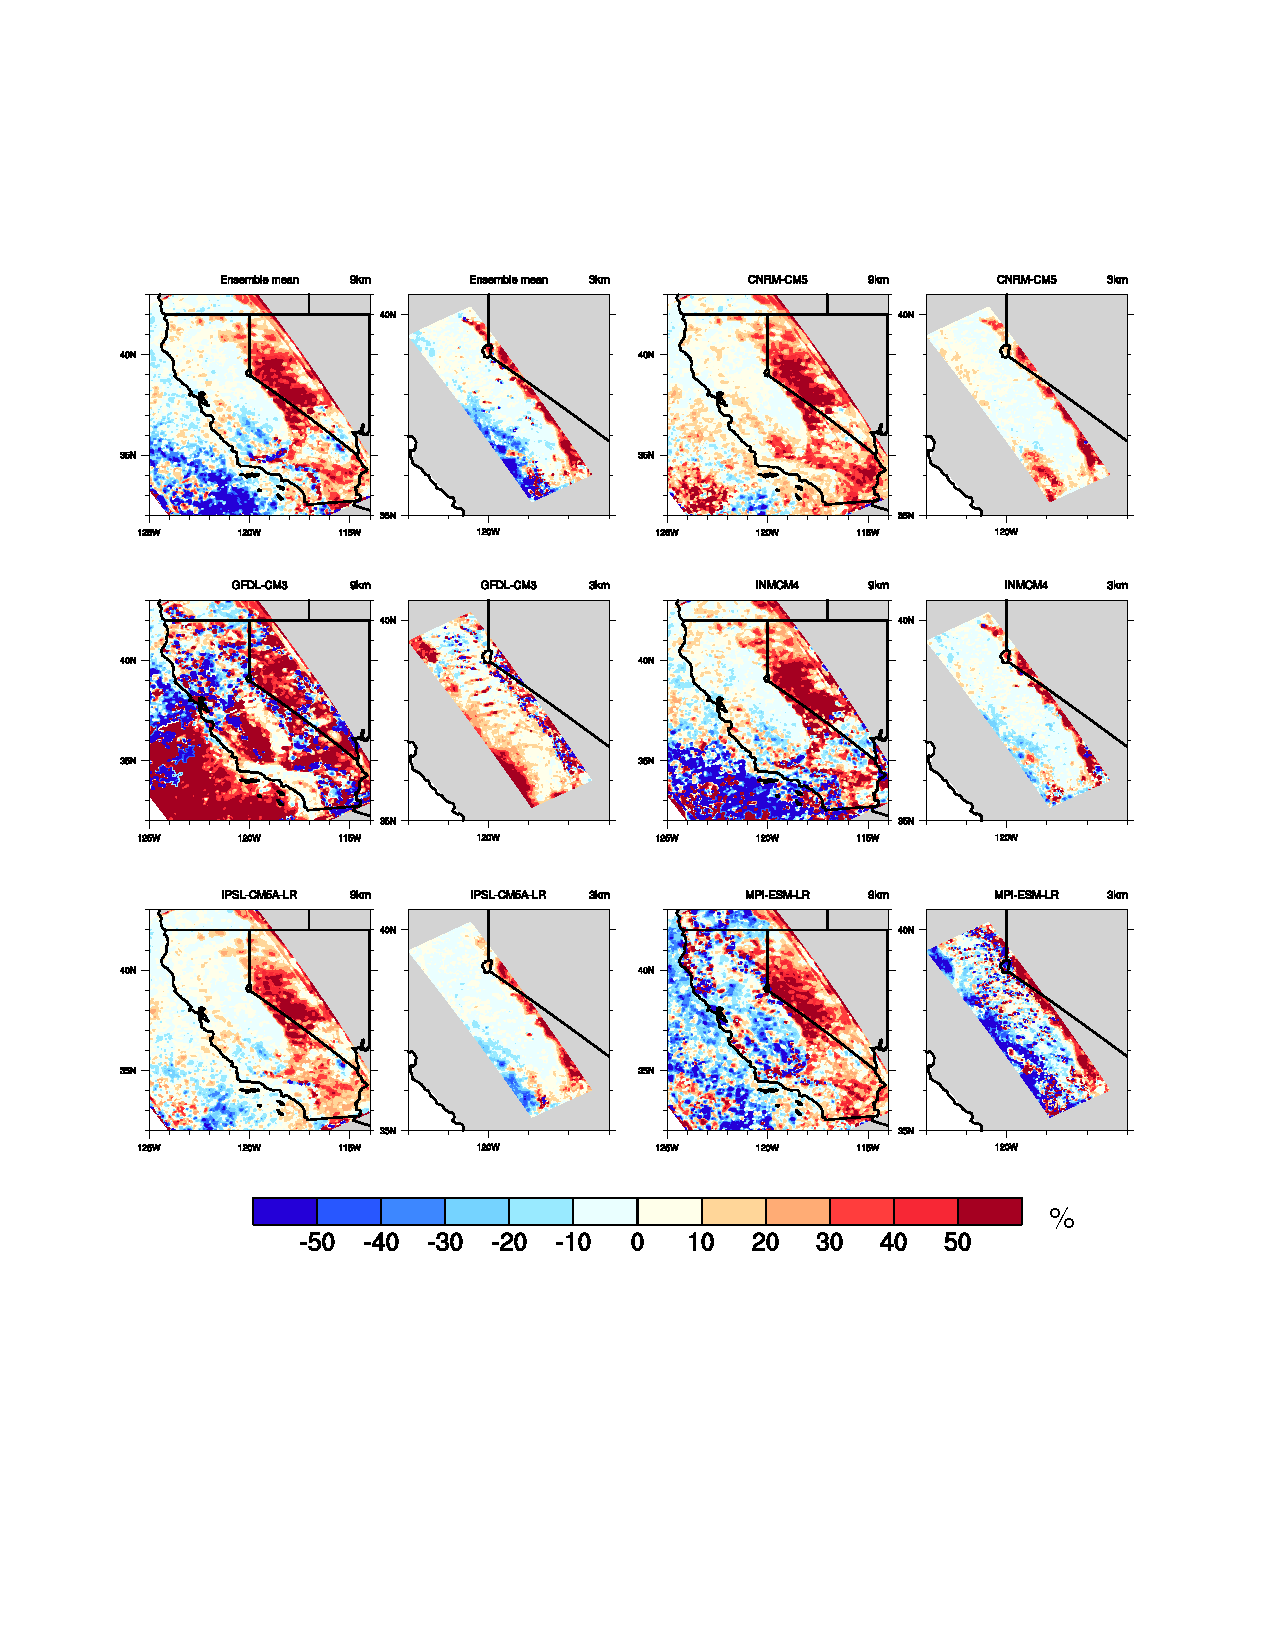
\includegraphics[width=6in]{R10_vs_pr_changes_DJF.pdf}
\caption{The relative contribution to the total precipitation changes resulted from the changes of low-rainy days (Pr$\leq$10mm/day).}
\label{fig:Figure 4}
\end{center}
\end{figure}

%the percentage of changes for the corresponding days are similar to this, also for Figure 5 and 6.

%Figure 5
\begin{figure}
\begin{center}
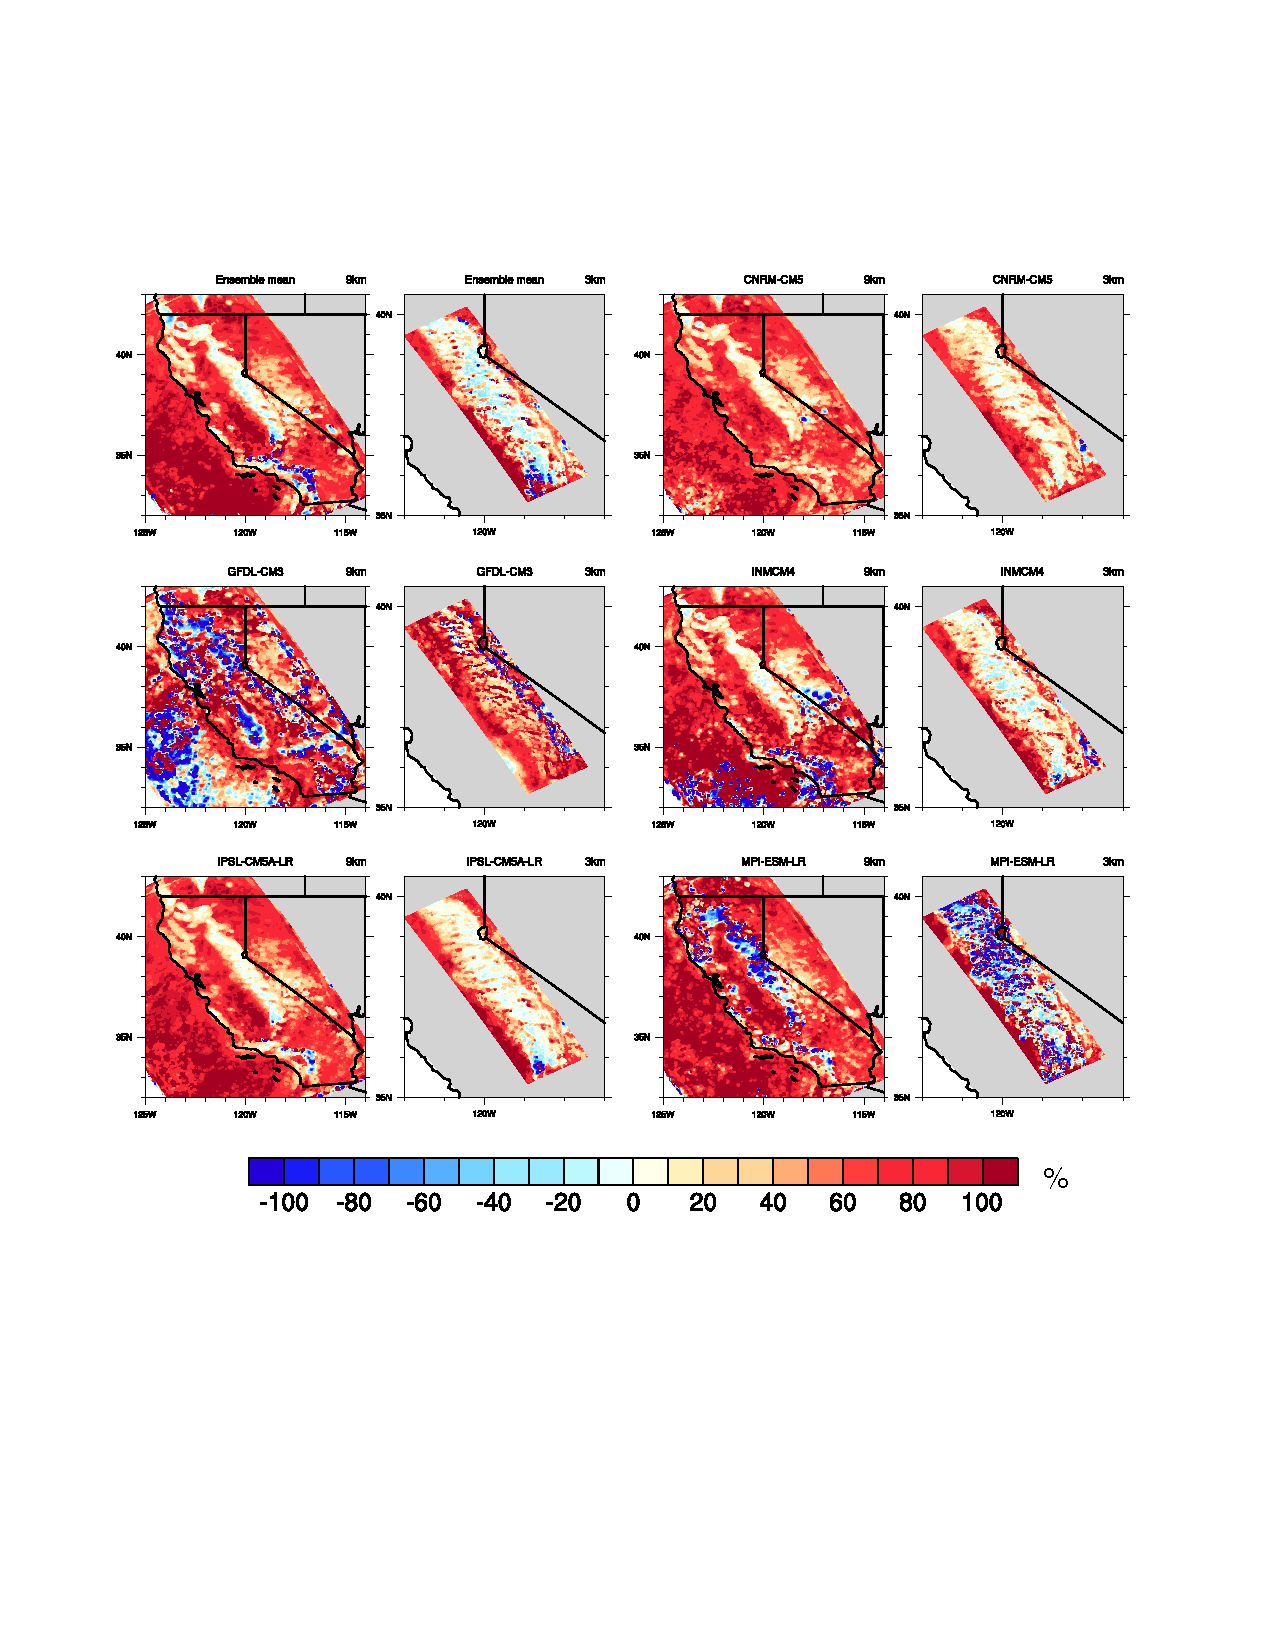
\includegraphics[width=6in]{R60_vs_pr_changes_DJF.pdf}
\caption{Similar as Figure 4 but for the high-rainy days (10mm$<$Pr$\leq$60mm/day).}
\label{fig:Figure 5}
\end{center}
\end{figure}

%Figure 6
\begin{figure}
\begin{center}
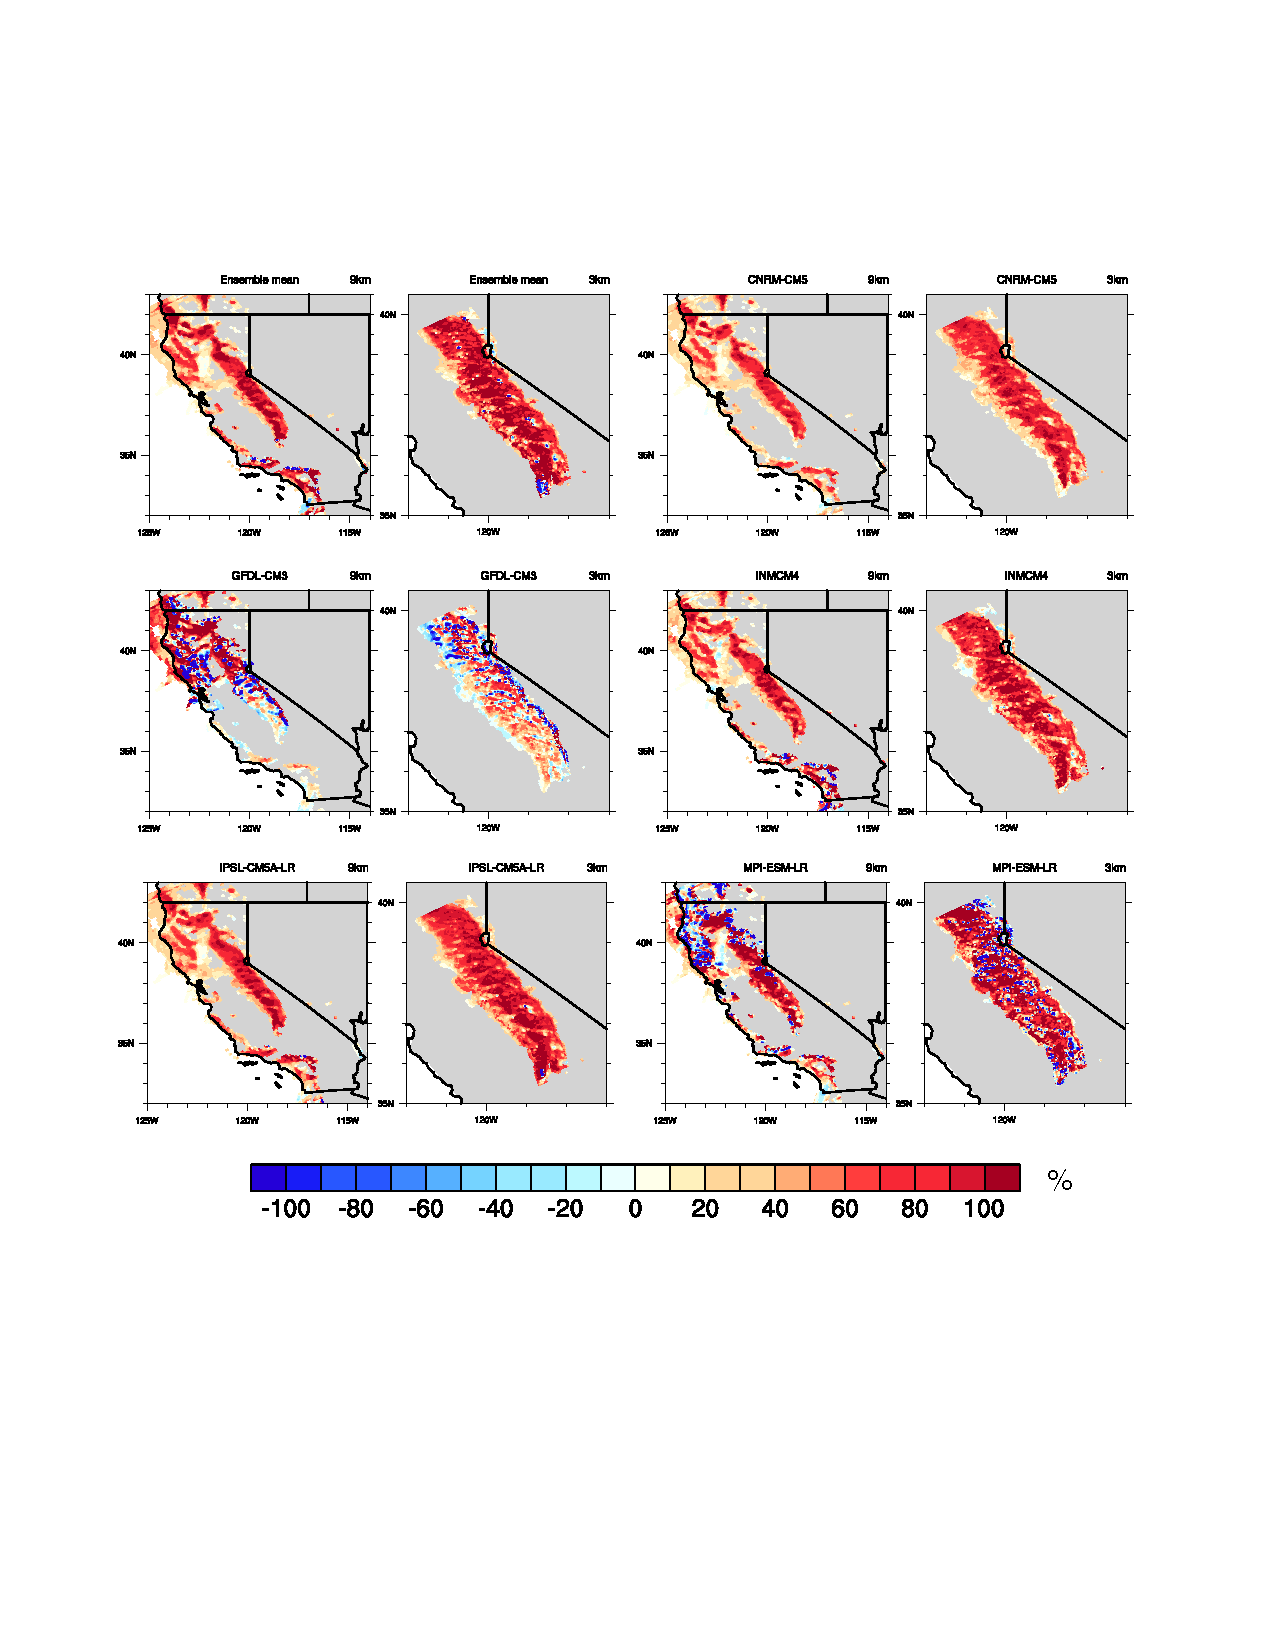
\includegraphics[width=6in]{Rxx_vs_pr_changes_DJF.pdf}
\caption{Similar as Figure 4 but for the precipitation extremes (Pr$>$60mm/day).}
\label{fig:Figure 6}
\end{center}
\end{figure}

%Figure 7
\begin{figure}
\begin{center}
\includegraphics[width=6in]{PDF_hist_DJF.pdf}
\caption{The frequency of the low-rainy, the high-rainy and the extreme over historical period (i.e. year 1991-2000) and their corresponding contributions to the total rainy amount.}
\label{fig:Figure 7}
\end{center}
\end{figure}

%Figure 8
\begin{figure}
\begin{center}
\includegraphics[width=6in]{Q2_future_vs_hist_relative_DJF.pdf}
\caption{The relative changes of the specific humidity compared to historical period.}
\label{fig:Figure 8}
\end{center}
\end{figure}

%Figure 9
\begin{figure}
\begin{center}
\includegraphics[width=6in]{Q2_vs_T2_changes.pdf}
\caption{The relative changes of the 2m specific humidity contrasted to the changes of 2m temperature.}
\label{fig:Figure 9}
\end{center}
\end{figure}

%Figure 10
\begin{figure}
\begin{center}
\includegraphics[width=6in]{R1mm_future_vs_hist_relative.pdf}
\caption{The relative changes of the rainy days during wet season (NDJFM) from past to future.}
\label{fig:Figure 10}
\end{center}
\end{figure}

%Figure 11
\begin{figure}
\begin{center}
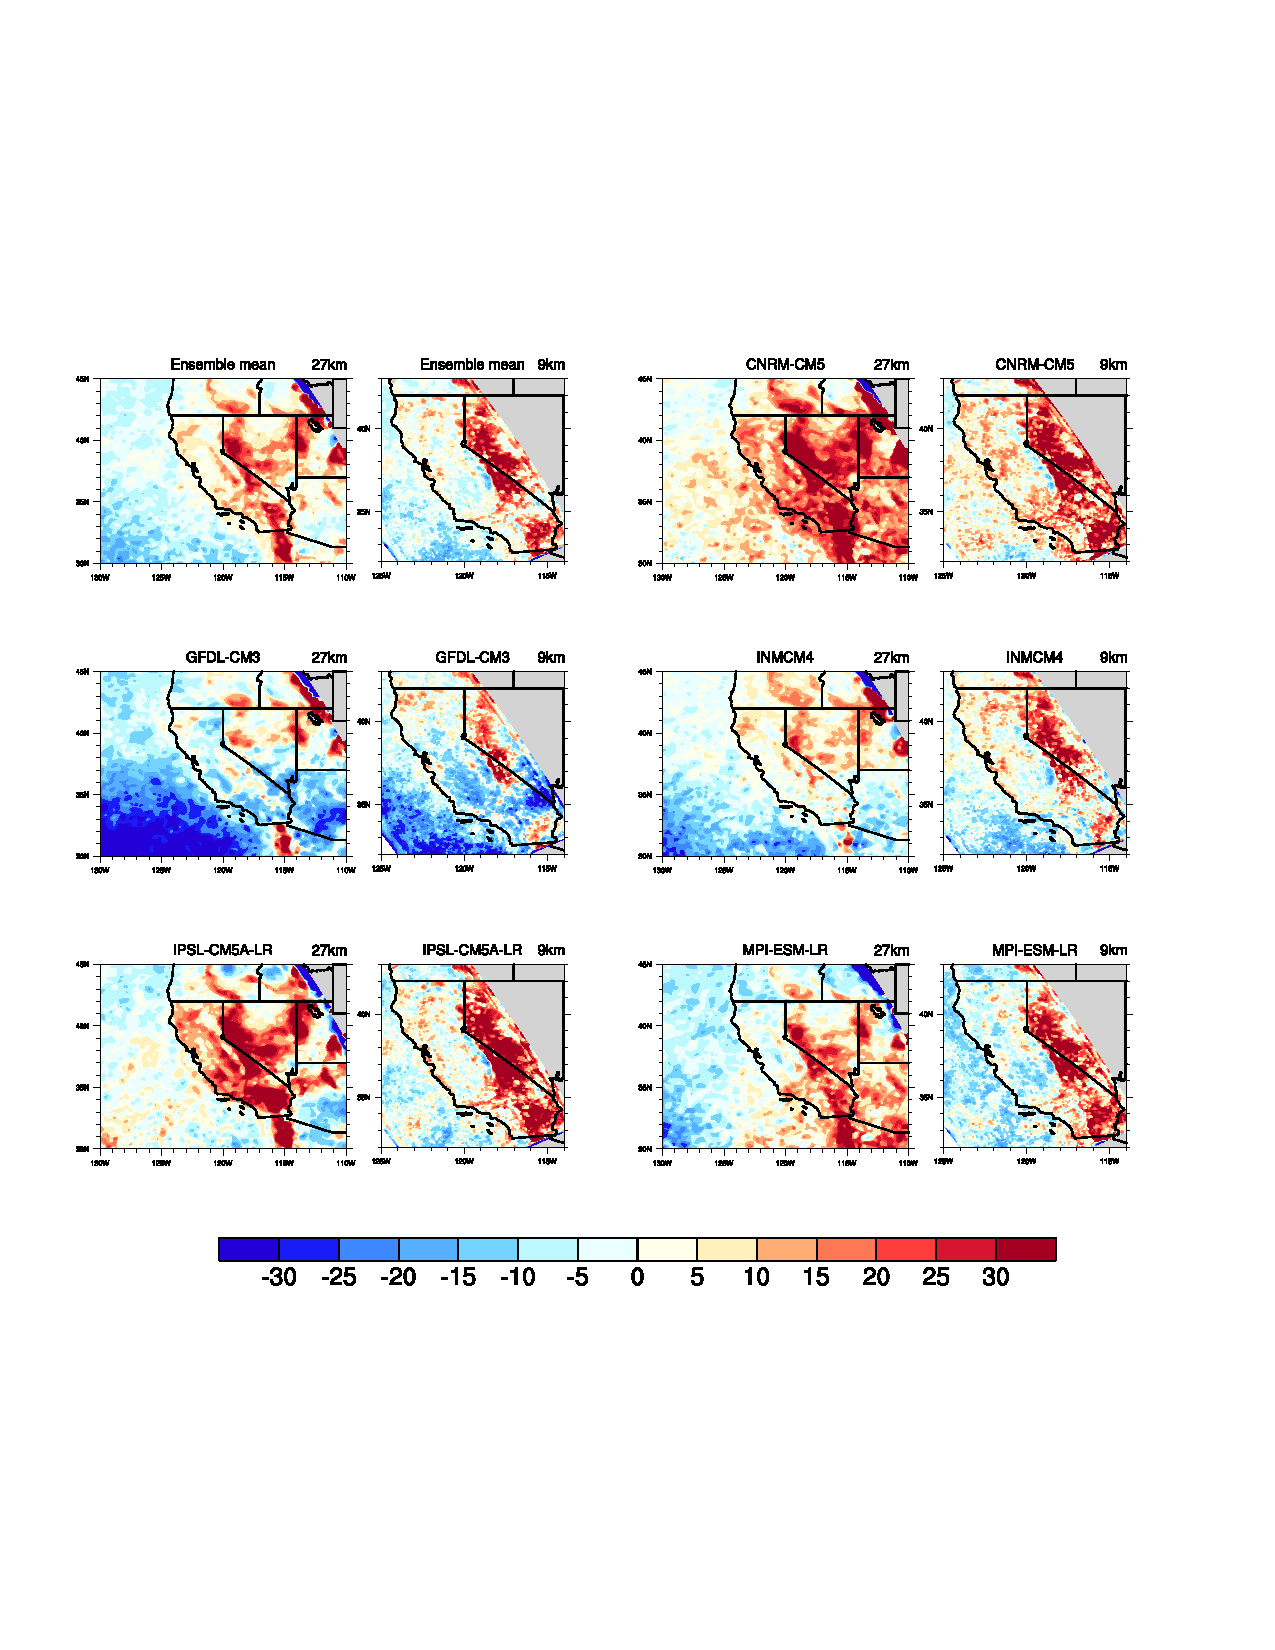
\includegraphics[width=6in]{R1to10mm_future_vs_hist_relative.pdf}
\caption{Similar as Figure 10, but for low-rainy days.}
\label{fig:Figure 11}
\end{center}
\end{figure}

%Figure 12
\begin{figure}
\begin{center}
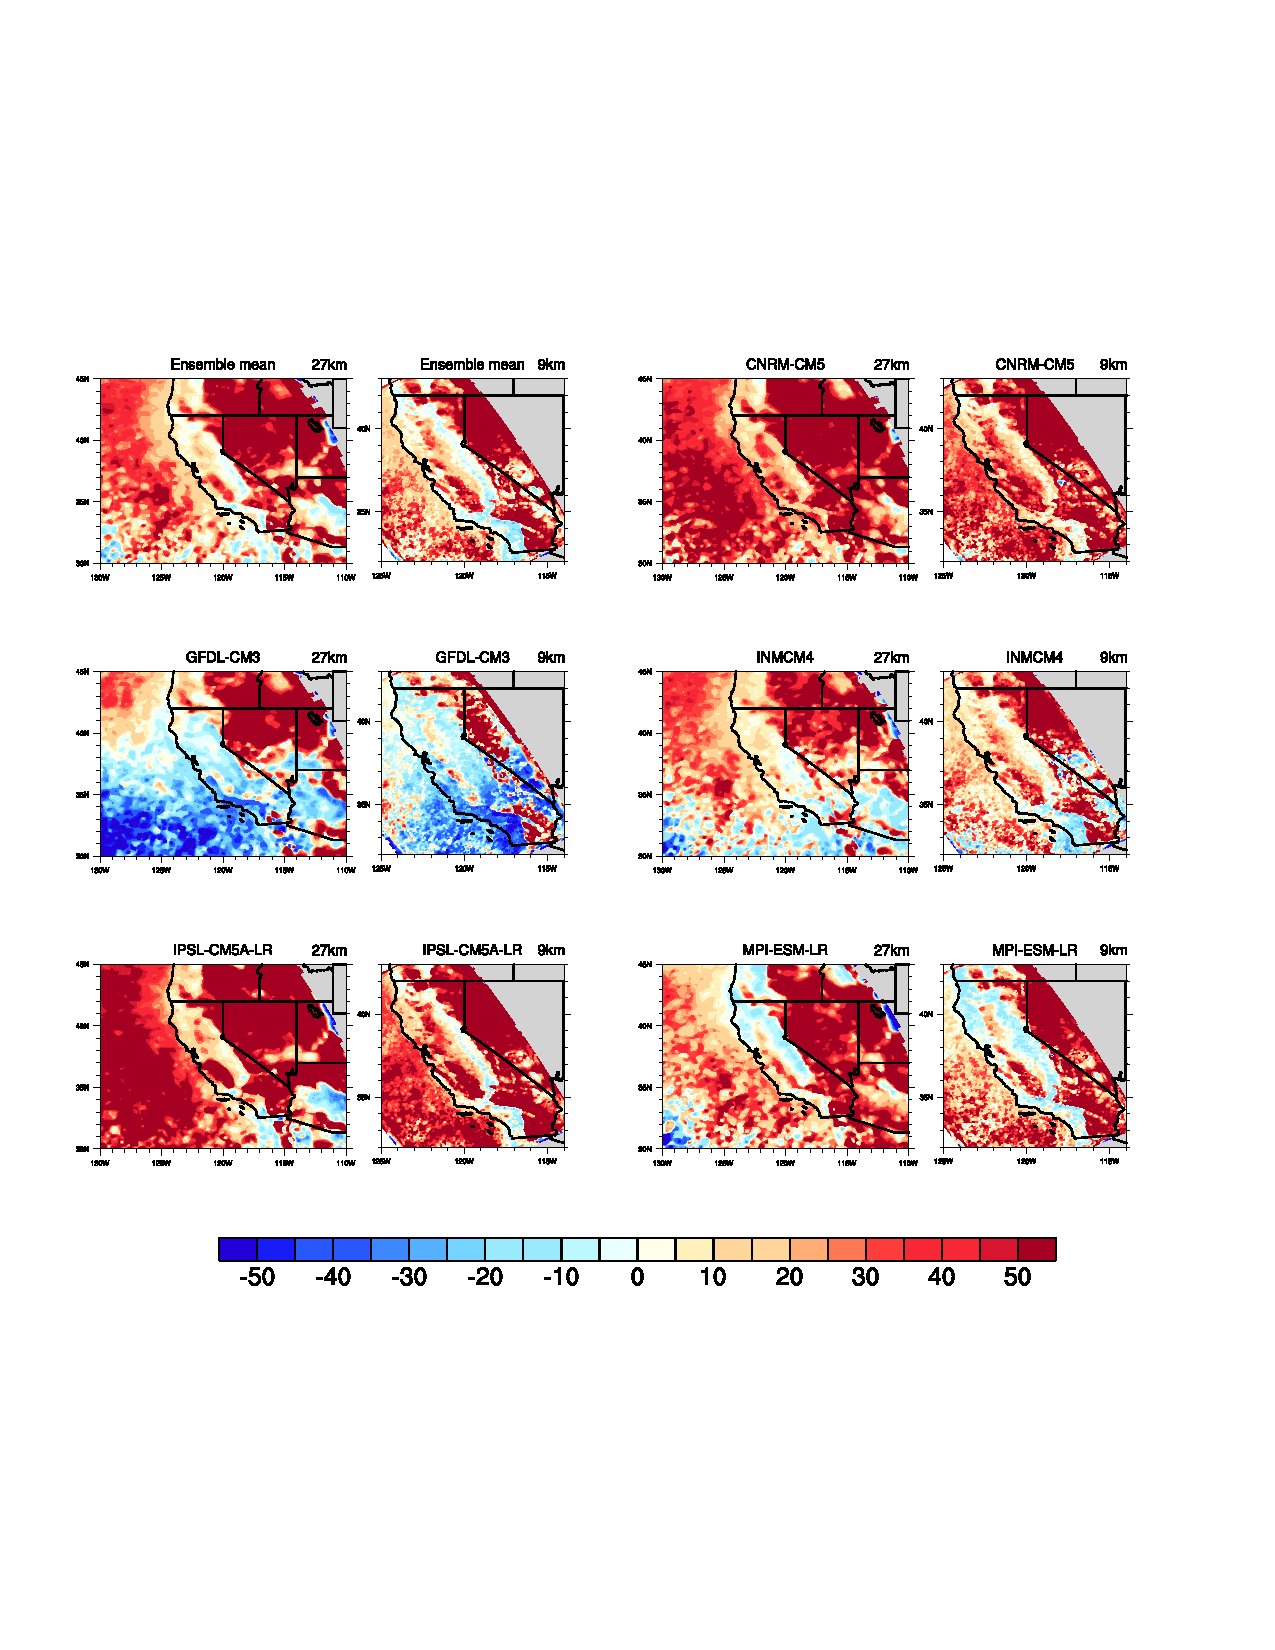
\includegraphics[width=6in]{R10to60mm_future_vs_hist_relative.pdf}
\caption{Similar as Figure 10, but for heavy-rainy days.}
\label{fig:Figure 12}
\end{center}
\end{figure}

%Figure 13
\begin{figure}
\begin{center}
\includegraphics[width=6in]{Rxx60mm_future_vs_hist_relative.pdf}
\caption{Similar as Figure 10, but for extremes.}
\label{fig:Figure 13}
\end{center}
\end{figure}


%Figure 14
\begin{figure}
\begin{center}
\includegraphics[width=6in]{P95_hist_future.pdf}
\caption{The 95th quantile (P95) of daily Pr at each grid point for hist and future at 9 km.}
\label{fig:Figure 14}
\end{center}
\end{figure}

%Figure 15
\begin{figure}
\begin{center}
\includegraphics[width=6in]{pr_pdf_divisions.pdf}
\caption{The frequency distribution of daily Pr ($>$1mm$/$day) based on all the grid points within different climate divisions for hist and future at 9 km. Note: (a) California, (b) Central Valley, (c) Mountain region, (d) Desert area, (e) North coast, (f) South coast.}
\label{fig:Figure 15}
\end{center}
\end{figure}

%Figure 16
\begin{figure}
\begin{center}
\includegraphics[width=6in]{Max1dPr_ivt.pdf}
\caption{The integrated water vapor transport (IVT) of the maximum 1 day Pr during the simulation periods for hist and future at 27 km.}
\label{fig:Figure 16}
\end{center}
\end{figure}

%Figure 17
\begin{figure}
\begin{center}
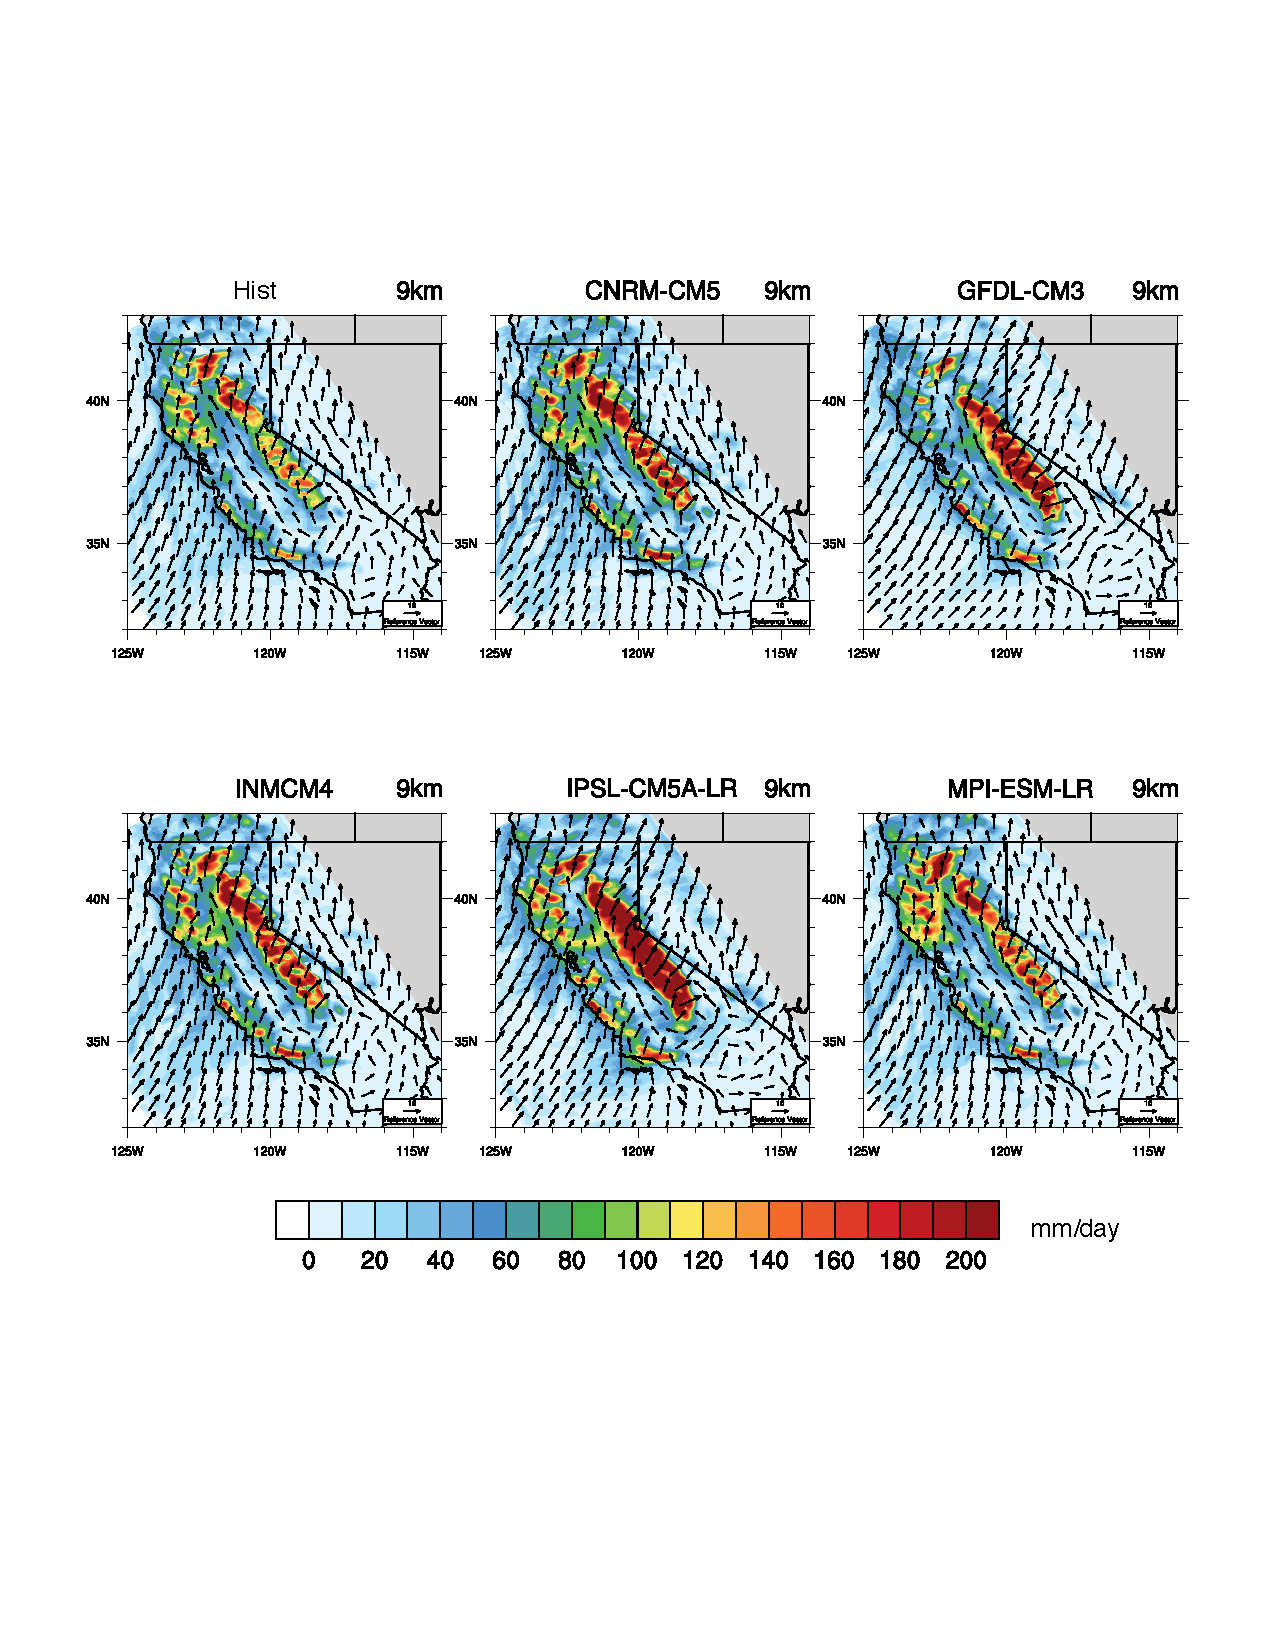
\includegraphics[width=6in]{Max1d_pr_uv10.pdf}
\caption{The near-surface wind pattern (at 10 m, unit: m/s) and Pr of the maximum 1 day Pr event for hist and future at 9 km.}
\label{fig:Figure 17}
\end{center}
\end{figure}

%Figure 18
\begin{figure}
\begin{center}
\includegraphics[width=6in]{ivt_gt_p95.pdf}
\caption{The average IVT and mean wind pattern as the mean Pr over CA exceeds the P95 value for hist and future at 27 km. Note: Here, the wind patterns for future simulations are the difference between specific future simulation and historical result.}
\label{fig:Figure 18}
\end{center}
\end{figure}

%Figure 19
\begin{figure}
\begin{center}
\includegraphics[width=6in]{ivt_gt_p85.pdf}
\caption{Similar as Figure 18, but for the case when Pr exceeds the P85 value.}
\label{fig:Figure 19}
\end{center}
\end{figure}


\end{document}
